\documentclass[oneside, notitlepage]{scrreprt}

\usepackage[english]{babel}
\usepackage{ucs}
\usepackage[utf8x]{inputenc}
\usepackage[bookmarksopen=true,
			bookmarks=true,
			plainpages=false,
        	pdfpagelabels=true,
			colorlinks=true,
			linkcolor=black,
			citecolor=black,
        	filecolor=black,
        	urlcolor=blue]{hyperref}
\usepackage{graphicx}
\usepackage{float}
\usepackage{listings}
\usepackage{color}
\usepackage{tikz}
\usepackage{scrpage2}

\lstdefinestyle{MyCStyle}{
  belowcaptionskip=1\baselineskip,
  breaklines=true,
  frame=single,
  captionpos=b,
  numbers=left,
  xleftmargin=\parindent,
  language=C,
  showstringspaces=false,
  basicstyle=\footnotesize\ttfamily,
  keywordstyle=\bfseries\color{green!40!black},
  commentstyle=\itshape\color{purple!40!black},
  identifierstyle=\color{blue},
  stringstyle=\color{orange}
}
\lstset{escapechar=@,style=MyCStyle}

\pagestyle{scrheadings}
\clearscrheadfoot
\clearscrplain
\setheadsepline{1pt}
\ohead{HTWG Konstanz}
\ihead{Fabian Meyer, Jens Gansloser}

\begin{document}

\title{Heart Rate Monitor}
\subtitle{Ubiquitous Computing Mini Project}
\author{Fabian Meyer \and Jens Gansloser}
\date{\today \\ HTWG Konstanz}
\maketitle

\begin{abstract}
The aim of this project is to build a heart rate monitor device. There are already a lot of devices commercially available which measure the heart rate. However, the internal functionality of these devices is not exposed to the user, so there cannot be made any statements about their precision and the quality of the results. Additionally, most devices need to be worn on the users chest or the user must place his finger on it. This document describes the principle and implementation of a heart rate monitor device, which is able to detect the heart rate with high precision and can be worn as a wrist band.
\end{abstract}
\clearpage

\tableofcontents

\chapter{Principle of Operation}
\label{chap:principle-of-operation}

There are several ways to measure the heart rate. This chapter describes the method used to get the heart rate data.

\section{Pulse Rate}
\label{sec:pulse-rate}
A method to measure the heart rate is the photoplethysmogram (PPG) technique. This method measures the change of the blood volume through the absorption or reflection of light. A light emitting diode (LED) shines through a thin amount of tissue (e.g. fingertip, earlobe). The wavelength of the light should be in near infrared area. On the other side a photodiode registers the intensity of light that traversed the tissue. Since blood changes its volume with each heart beat, more or less light of the LED gets absorbed by it. If the heart pushes blood through the vessels, more blood lays between the LED and photodiode. As a result the registered intensity of light changes continuously with the pulse. By measuring the time between two intensity peaks the current pulse can be estimated. The setting for the pulse rate monitor is displayed in figure \ref{fig:pulse-rate-monitor-setting}.

\begin{figure}[H]
	\centering
	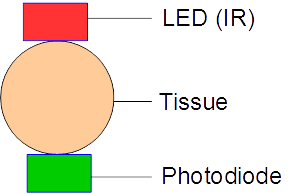
\includegraphics[width=180px]{images/pulse-rate-aufbau.png}
	\caption{Pulse Rate Monitor Setting - Light through skin}
	\label{fig:pulse-rate-monitor-setting}
\end{figure}

An alternative way to measure the heart rate is to detect the reflected light. The LED and the photodiode can be placed on the same side. This setting is displayed in figure \ref{fig:pulse-rate-monitor-setting2}

\begin{figure}[H]
	\centering
	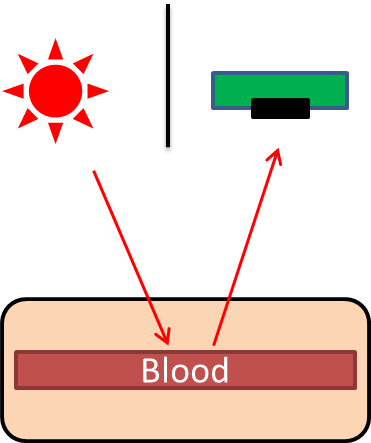
\includegraphics[width=130px]{images/pulse-rate-aufbau2.png}
	\caption{Pulse Rate Monitor Setting - Light reflected}
	\label{fig:pulse-rate-monitor-setting2}
\end{figure}

\section{Oxygen Saturation}
\label{sec:oxygen-saturation}
The oxygen saturation of the blood can be measured by using 2 light emitting diodes. One LED emits light with a wavelength of 660nm (red light), the other emits light with a wavelength of 940nm (infrared light). The absorption of light by blood changes corresponding to its oxygen saturation. Oxygenated blood absorbs more infrared light and less red light. With de-oxygenated blood it is the other way around \cite{bib:pulse-oximetry}. The LEDs blink alternating and a photodiode is used to measure the light intensity after the light traversed the tissue. These measurements in combination with the Lambert-Beer-Law are used to calculate the oxygen saturation.

\chapter{Environment}
\label{chap:environment}

This chapter describes the hardware and the software used and implemented for the project. Figure \ref{fig:data-flow} shows the different hardware parts and how they interact with each other. Note that the displayed setting is different from the actual used one in the prototype due to wrong hardware orders. The prototype setting is explained in chapter \ref{chap:hrm}.

\begin{figure}[H]
	\centering
	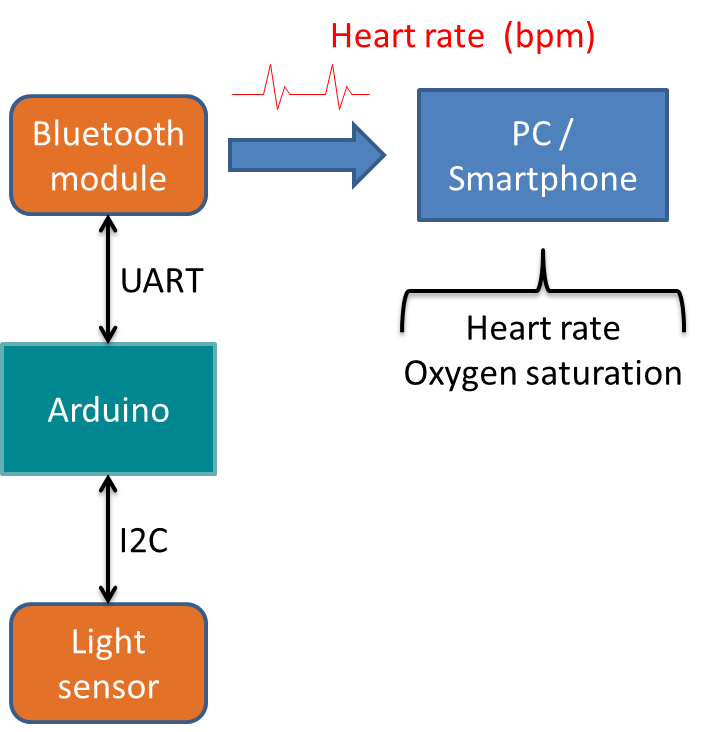
\includegraphics[width=200px]{images/general_dataFlow.png}
	\caption{Project setup}
	\label{fig:data-flow}
\end{figure}

\section{Hardware}
\subsection{Light Intensity Sensor}
\label{subsec:light-intensity-sensor-hardware}

To measure light, the 16bit TSL2561 Luminosity Sensor breakout board from Adafruit is used. It provides the TSL2561 Light-To-Digital Converter which is able to sense full spectrum and IR light with a very high sensitivity (see graphic below). The sensor contains of a broadband photodiode (visible and infrared) and a infrared photodiode. Two ADCs convert the analog data to digital data, that can be read via the I$^{2}$C bus. The light sensor can be configured with different gain, which changes the sensitivity to light. This is needed if the sensor is used in areas with bright light or low light. A second option to configure is the integration time (13ms, 101ms, 402ms). This configures the resolution of the device, so that the sensor has more time to take samples. With a integration time of 402ms, the sensor has the complete 16bit resolution. The output of the sensor can be used to calculate the measured SI-Unit lux, which indicates the illuminance \cite{bib:tsl-sensor}. Figure \ref{fig:tsl-2561-spectrum} shows the light spectrum of the two photodiodes on the board.

\begin{figure}[H]
	\centering
	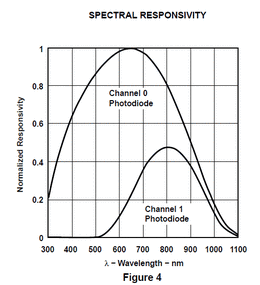
\includegraphics[width=200px]{images/light_tsl2561spectrum.png}
	\caption{TSL-2561 Spectrum}
	\label{fig:tsl-2561-spectrum}
\end{figure}

\subsection{Microcontroller}
\label{subsec:microcontroller}
The data of the sensor is further computed by an Arduino \cite{bib:arduino-board}. The Arduino receives the data of the sensor via I$^{2}$C bus system. Different Arduinos can be used. The only requirement is, that the Arduino has an I$^{2}$C and UART (Bluetooth) interface to communicate with the light sensor and the PC/Smartphone.

\subsection{Bluetooth Module}
\label{subsec:bluetooth-adapter-hardware}
The Bluefruit EZ-Link is a serial link bluetooth module. That means, the Arduino can communicate via UART with the bluetooth module, which handles the wireless transmission to the computer. On the computer side, the module (if it was paired successfully) is recognized as an serial port (COM). See also \cite{bib:bluetooth-adapter}.

\section{Libraries}
To create the heart rate monitor, several external libraries were used. This section lists all used external libraries and explains its usage.

\subsection{FFTW}
FFTW is a C library, which offers functions to calculate the discrete Fourier Transform (DFT). It supports the calculation with multiple dimensions, complex or real data and different input sizes. HRM uses FFTW to compute the complex DFT of the light sensors values and determine than the heart rate.

\subsection{Qt}
Qt is a cross-platform library to create Graphical User Interfaces. Additionally, it supports own container classes, networking, database access and a lot of more. For the HRM, Qt is used to create the GUI.

\subsection{Qwt}
Qwt is a add-on for Qt which is able to create 2D and 3D plots. Its advantages are the large amount of features and the high performance. This makes it suitable for technical applications, which need to display a lot of data. Qwt is used to plot the light sensors data and its Fourier Transformed.

\subsection{QtSerialPort}
QtSerialPort is used to access the serial port from the PC. It is a add-on module for Qt4 and Qt5. It allows fast and easy writing and reading to the serial ports. Because Qt is used for the Graphical User Interface (GUI), this is the optimal solution for serial port access.

\section{Heart Rate Monitor Software}
This section shows all implemented modules which are part of HRM. The implementation details are outlined in chapter \ref{chap:impl-details}.

\subsection{Graphical User Interface}
The GUI is mainly used for debugging and optimization. The GUIs features are shown in the following list:

\begin{itemize}
	\item{Displays the received data from the Arduino (via serial port)}
	\item{Displays the light sensors settings}
	\item{Allows setting of the light sensors sample rate}
	\item{Displays several diagrams (sensor values, frequency spectrum, ...}
	\item{Displays the Signal Processing parameter}
\end{itemize}

\subsection{Serial Interface}
The class \lstinline{Serial} is used to control the access to the serial port. Qts slot and signal mechanism is used, to notify other classes, that data is received. The class supports sending and receiving data. The following signals are available for receiving plain string data, the light sensors luminosity values or its settings.

\begin{lstlisting}
signals:
    void receiveLine(QString data);
    void receiveSensorData(SensorData data);
    void receiveSensorSettings(SensorSettings settings);
\end{lstlisting}

The sensor settings are saved in the following struct.

\begin{lstlisting}
struct SensorSettings {
    QString sensor;
    QString id;
    QString max;
    QString min;
    QString resolution;
    QString sampleInterval;
};
\end{lstlisting}

The light sensor data is saved in the \lstinline{SensorData} structure.

\begin{lstlisting}
struct SensorData {
	uint16_t broadband;
	uint16_t ir;
};
\end{lstlisting}

Sending data to the Arduino is done with the \lstinline{void sendData(QString string);} function.

\subsubsection{Serial Configuration}
The following serial port configuration is used:
\begin{itemize}
	\item{Port Name: /dev/ttyACM0}
	\item{Baudrate: 9600}
	\item{Data Bits: 8}
	\item{Parity: No}
	\item{Stop Bit: 1}
	\item{Flow Control: No}
\end{itemize}

\subsection{Signal Processing Module}

\subsection{Arduino Module}

\subsection{Light Intensity Sensor}
\label{subsec:light-intensity-sensor-software}
To get data from the light sensor, the Adafruit TSL2561 and Adafruit Unified Sensor Driver library are used. These libraries do the I$^{2}$C communication and the digital to lux calculation. Also they provide functions to set the gain and integration time options. \cite{bib:tsl-library} \cite{bib:sensor-library}

\begin{lstlisting}[caption=Adafruit driver]
tsl.enableAutoRange(true);
tsl.setIntegrationTime(TSL2561_INTEGRATIONTIME_13MS);

uint16_t broadband, ir;
tsl.getLuminosity(&broadband, &ir);
\end{lstlisting}

Line 1 sets the gain value to auto range. That means it adapts automatically to the sensors environment. On line 2 the integration time is set to 13ms (low resolution, fast processing). Line 5 queries for the luminosity values of the broadband and ir photodiode. For the use in this project, the sensor driver had to be slightly modified to allow manual integration times. The original driver allows only to set three different static integration times (13ms, 101ms, 402ms). Specific integration time are required to allow the desired sample frequencies. The extended driver provides functions to start and stop the integration of the light values, shown in the following code extract.

\begin{lstlisting}[caption=Adafruit\_TSL2561\_U.h]
/* Manual timing control */
void beginIntegrationCycle();
void stopIntegrationCycle(uint16_t *broadband, uint16_t *ir);
\end{lstlisting}

\chapter{Heart Rate Monitor}
\label{chap:hrm}

\section{Solution Approach}
Figure TODO shows the output signal from the light sensor. The diagramm shows the different luminosity values over time (= heart rate) of a patient.
It measured by placing the finger between the light sensor and the LED.

PICTURE

To get now the exact heart rate, the time between two minima of the discrete sensor value need to be determined. However, it is not trivial to determine
the minima, because of the noise in the signals data. The noise comes from different environment settings, the difference in blood volume change of each person and
how the finger is placed onto the sensor. These paramter result in a change in they datas Y Part.

\subsection{First Approach}
A first naive approach is, to determine the grade of each sample point in the input data and than look, if the curve is declining or risings.
With this knowledge, the minima can be identified. This approach is not optimal. It is impossible to seperate different minimas in the data and find the correct ones.
Due to the noise, there can be local minimas/optimas which are not needed. Introducing a static limit is unsuitable too, because in the difference of the y-axis data in each sample.
To conclude, this approach is not suitable for the problem.

\subsection{Second Approach}
As one can see in figure TODO, the heart rate is represented by a periodic up and down of the input values. These up and down values are disorted by some noise.
Viewed from a signal processing view, these up and downs have the highes contribution of frequencies to the input signal. To get the heart rate, the highest frequency (= heart rate)
of the input signal has to be determined. This is a perfect application field for the Fourier Transformation. The Fourier Transformation is a mathematical method to analyse a
input signal and determine the different frequencies which contribute how much to this signal. A Forier Transformation converts an input signal in the time domain to an output signal in the
frequency domain. The output signal shows, how much each frequency contrinutes to the input signal. The basic idea is, to transform the input signal via the Fourier Transformation and than
determine the signal which contirubutes most. These means determineing the peak of the output frequency signal. Picture TODO shows the basic operation principle.

\section{Data Flow}

\section{Signal Processing}

\subsection{Fourier Transformation}
There are a lot of different kinds of Fourier Transformation for different application fields. First, the correct kind has to be determined.
Fourer Transformation can be used for analysis and sythesis. Because we want to get the frequency domain signal from the time domain signal,
we use the forward transform. Beacus the input signal is an array of discrete vaklues, the discrete FT is need. The formula for the DFT is showin in.
As shown, complex numbers are used. The input are sicrete input values x[n]. The output are complex discrete values X[k].
An fast implementation of the FT is the FFT. The FFTW library is used to compute the FFT of the sebnsors data.

Also the FT is the basic principle to get the heart rate, additional steps need to be made to get a nice frequency spectrum. The following chapters describe
the different steps in detail. Figure TODO shows the applied functions.

\subsubsection{Window Function}
To reduce the leakage-effect, a window function has to be applied. The leakage effect artifacts in discrete FTs. It happens when TODO:(basic frequency).
This is because an input signal is normally not periodic. These input window cuts the signal data at the start and end. The resulting output frequency
domain is convoluted (smeared). In other words, when applying the FT, it assumes that the input signal is peridoc by queueing multiple of these windows at it each other.
However, because there are no consistent cuts at the start and end, the window sequence does not fit good. To reduce this effect, a window function needs to be applied.
This window function is multiplied with the input signal. It reduces the value at each side of the input data to zero, the windows fit perfectly to each other
(when they are added to a sequence). There are different window functions to choose from. The used function is the Hamming-Window, which TODO.
An improvement is a slightly modiefied version of the hamming window.

\subsubsection{FFT}
Now the FFT can be applied, to transform the data into the frequency domain. This is done by the FFTW library. The input data is the discrete light data array with N values.
Because the discrete complex FT (DFT) works with complex numbers, the complex part of each inout element is set to 0. The output of the FFT is also an array of N complex numbers.

\subsubsection{Filter}
When applying the steps mentioned above (Window Function, FFT), the output signal looks like shown in Figure TODO. There are a lot of high Frequencies and it is difficult to find
the right optimum (Figure, peak symbol). The low frequencies are from the noise. To remove these unwanted frequencies, a bandpass filter is applied. To measure the heart rate, only heart rates from
40 - 230bpm are possible (normally). This means, only frequnecies from 0.7 - 3.9Hz need to be identified. All other frequencies in the input signal can be removed. To this, a perfect bandpass filter
which only allows the desired frequencies is used. The filter can be applied to the input signal (convoluting with e.g. butterworth bandpass filter) or to the output signal (multiplication - cutting the unwanted frequencies). Because the second option is much miore faster and allows to use a perfect filter, this option is used.

\subsubsection{Converting/Scaling}
The resulting frequency domain values need to be scaled, to represent the correct amplitude. This is made by the following formula (TODO).
The output format is displayed in the following figure (TODO). The first element of the array represents the DC offset (y-axis shift) and is not needed.
This is because this valuie changes based on the noise/environment light. The next 1 - n/2 values represent the positive frequencies. The other values the negatkve frequencies.
For this applicatio, only the positive frequencies are used. So only the first half elemens (1 - N/2) need our attention. These values are complex values (sin and cos) are in rectangular coordinated and need to be converted in polar coordinated, to make it more human readable. Only the magnitude of this data is important, t o calculate the heart rate.

Additionally, because the filter needs some time until it is stabilized, the stabilization time has to be cut of from the signal. Else, this would result in bad output data.

\subsubsection{Peak Detection}
The last step to do is to detect the peak. This is be done by iterating through the magnitude values and find the the value (x-value) with the highest aplitude.
These x-value needs to be converted into beats per minute, the standard heart rate unit.

\subsection{Parameters}
Additionally to applying the different signal processing steps, the correct paramters need to choosen. There are several requirements to the signal processing:
\begin{itemize}
	\item{Small number of samples used for FFT (else it will take long time until enough data is gathered)}
	\item{High frequency resolution (0.1bpm)}
	\item{Fast calulcation (for implementing on smartphone/uC/...)}
	\item{Nice output data in frequency domain which allows easy peak detection}
\end{itemize}

\subsubsection{Sample Rate}
To detect frequencies up to 4Hz, a minimal sample rate of 8Hz (Shannon-Nyquist theorem) is required.
This means a minimal sample interval of 125ms is required. The light sensor allows sample intervals up to 15ms.

\subsubsection{Frequency Resolution}
An optimal value for the number of samples are 128. It allows a good tradeoff between frequency resolution and required sample time.
However, the frequency resolution is not good enough (3.75bpm). To further improve the resolution, the following steps can be made:

\begin{itemize}
	\item{More samples (unsuitable, because requires more time)}
	\item{Zero Padding (interpolating by adding zeros to the end of the input data). However, its only a trick, because it adds not more information to the data.}
	\item{Higher sample rate. A higher sample rate results in more frequencies that can be detected. The filter can remove them.}
\end{itemize}

\subsubsection{Data Segment}
To get continues frequency spectrums, the FFT is applied to the 128 samples every 5 samples. This is called segment duration. It means, that every 5 samples, the FFT of the last 128 samples is calculated.
The segment duration of 5 is trade off between fast results and required computation time. Else, the user has to wait 128 (= TODO, s) until he gets a new frequency spectrum and therefore a heart rate value.
To implement this, special buffer was created, which allows using different segment durations and fast data aquiring.

\chapter{Critique and Improvements}
Based on this work, a lot of projects can be done, to improve the heart rate monitor.

\begin{itemize}
	\item{Porting to a Arduino}
	\subitem{FFT library is available}
	\subitem{Performance tests need to be made}
	\item{Using a smartphone for signal processing}
	\item{Porting to a smaller uC.}
	\item{Adding a bluetooth module (trivial)}
	\item{Add oygen saturation measurement}
	\subitem{Easy to implement with the existing knowledge}
	\item{Create a wrist band}
	\item{Brighter LED}
	\item{Better light sensor (more sensitive)}
\end{itemize}

\chapter{Implementation Details}
\label{chap:impl-details}

\section{Wiring}
\label{sec:wiring}
TODO: Picture

\begin{thebibliography}{999}
	\bibitem{bib:pulse-oximetry} Pulse Oximetry, Dr. Chloe Borton, \url{http://www.patient.co.uk/doctor/pulse-oximetry}, 30.05.2014
	\bibitem{bib:tsl-sensor} TSL2561, \url{https://learn.adafruit.com/tsl2561/overview}, 30.05.2014
	\bibitem{bib:arduino-board} Arduino Board, \url{http://www.adafruit.com/product/50}, 31.05.2014
	\bibitem{bib:bluetooth-adapter} Bluefruit EZ-Link, \url{https://learn.adafruit.com/introducing-bluefruit-ez-link/overview}, 31.05.2014
	\bibitem{bib:tsl-library} TSL 2561 Library, \url{https://github.com/adafruit/Adafruit_TSL2561}, 31.05.2014
	\bibitem{bib:sensor-library} Adafruit Unified Sensor Driver library, \url{https://github.com/adafruit/Adafruit_Sensor}, 31.05.2014
\end{thebibliography}

\cleardoublepage
\addcontentsline{toc}{chapter}{\listfigurename}
\listoffigures

\end{document}